\documentclass{standalone}
\usepackage{tikz}
\usetikzlibrary{patterns, positioning}

\begin{document}
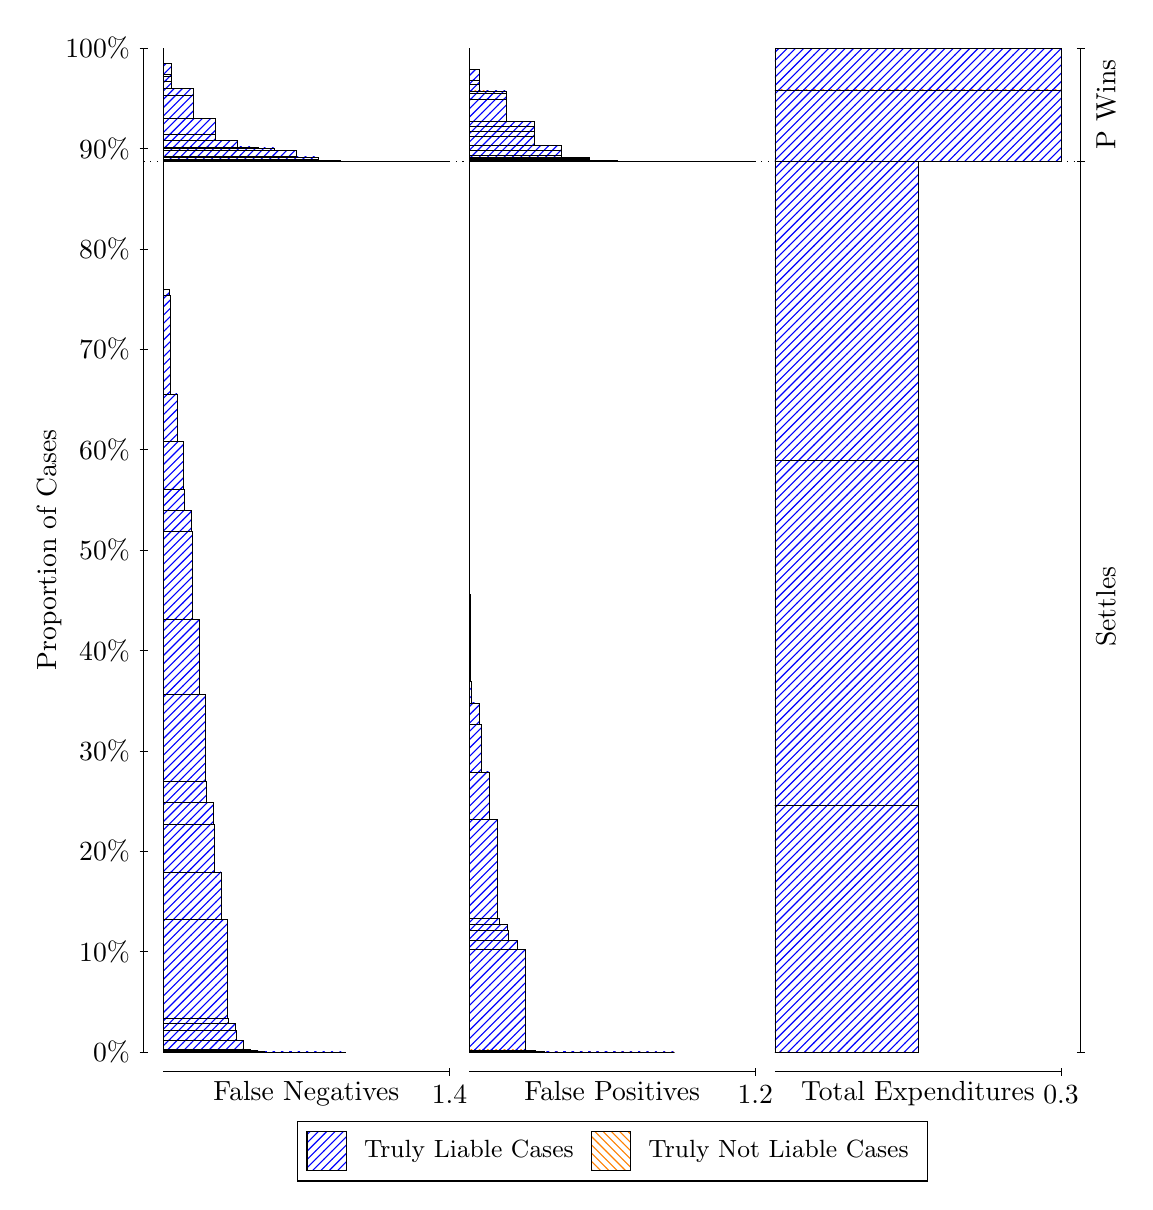
\begin{tikzpicture}
\draw[black, very thin] (1.5,1.75) -- (1.5,14.5);
\node[rotate=90, anchor=center] at (0.3, 8.125) {Proportion of Cases};
\draw[black, very thin] (1.45,1.75) -- (1.55,1.75);
\node[anchor=east] at (1.45, 1.75) {0\%};
\draw[black, very thin] (1.45,3.025) -- (1.55,3.025);
\node[anchor=east] at (1.45, 3.025) {10\%};
\draw[black, very thin] (1.45,4.3) -- (1.55,4.3);
\node[anchor=east] at (1.45, 4.3) {20\%};
\draw[black, very thin] (1.45,5.575) -- (1.55,5.575);
\node[anchor=east] at (1.45, 5.575) {30\%};
\draw[black, very thin] (1.45,6.85) -- (1.55,6.85);
\node[anchor=east] at (1.45, 6.85) {40\%};
\draw[black, very thin] (1.45,8.125) -- (1.55,8.125);
\node[anchor=east] at (1.45, 8.125) {50\%};
\draw[black, very thin] (1.45,9.4) -- (1.55,9.4);
\node[anchor=east] at (1.45, 9.4) {60\%};
\draw[black, very thin] (1.45,10.675) -- (1.55,10.675);
\node[anchor=east] at (1.45, 10.675) {70\%};
\draw[black, very thin] (1.45,11.95) -- (1.55,11.95);
\node[anchor=east] at (1.45, 11.95) {80\%};
\draw[black, very thin] (1.45,13.225) -- (1.55,13.225);
\node[anchor=east] at (1.45, 13.225) {90\%};
\draw[black, very thin] (1.45,14.5) -- (1.55,14.5);
\node[anchor=east] at (1.45, 14.5) {100\%};

\draw[black, very thin] (13.4,1.75) -- (13.4,14.5);
\draw[black, very thin] (13.35,1.75) -- (13.45,1.75);
\node[anchor=west] at (13.35, 1.75) {};
\draw[black, very thin] (13.35,13.062) -- (13.45,13.062);
\node[anchor=west] at (13.35, 13.062) {};
\draw[black, very thin] (13.35,14.5) -- (13.45,14.5);
\node[anchor=west] at (13.35, 14.5) {};

\draw[black, very thin, pattern color=blue, pattern=north east lines] (1.75,1.75) rectangle (4.0678,1.75);
\draw[black, very thin, pattern color=blue, pattern=north east lines] (1.75,1.75) rectangle (3.7894,1.75);
\draw[black, very thin, pattern color=blue, pattern=north east lines] (1.75,1.75) rectangle (3.692,1.75);
\draw[black, very thin, pattern color=blue, pattern=north east lines] (1.75,1.75) rectangle (3.511,1.75);
\draw[black, very thin, pattern color=blue, pattern=north east lines] (1.75,1.75) rectangle (3.4135,1.75);
\draw[black, very thin, pattern color=blue, pattern=north east lines] (1.75,1.75) rectangle (3.3161,1.7501);
\draw[black, very thin, pattern color=blue, pattern=north east lines] (1.75,1.7501) rectangle (3.2326,1.7502);
\draw[black, very thin, pattern color=blue, pattern=north east lines] (1.75,1.7502) rectangle (3.1351,1.7502);
\draw[black, very thin, pattern color=blue, pattern=north east lines] (1.75,1.7502) rectangle (3.0377,1.7568);
\draw[black, very thin, pattern color=blue, pattern=north east lines] (1.75,1.7568) rectangle (2.9542,1.7625);
\draw[black, very thin, pattern color=blue, pattern=north east lines] (1.75,1.7625) rectangle (2.9402,1.7738);
\draw[black, very thin, pattern color=blue, pattern=north east lines] (1.75,1.7738) rectangle (2.8567,1.7793);
\draw[black, very thin, pattern color=blue, pattern=north east lines] (1.75,1.7793) rectangle (2.7593,1.9022);
\draw[black, very thin, pattern color=blue, pattern=north east lines] (1.75,1.9022) rectangle (2.6757,2.0235);
\draw[black, very thin, pattern color=blue, pattern=north east lines] (1.75,2.0235) rectangle (2.6618,2.1083);
\draw[black, very thin, pattern color=blue, pattern=north east lines] (1.75,2.1083) rectangle (2.5783,2.1821);
\draw[black, very thin, pattern color=blue, pattern=north east lines] (1.75,2.1821) rectangle (2.5644,3.4343);
\draw[black, very thin, pattern color=blue, pattern=north east lines] (1.75,3.4343) rectangle (2.4808,4.0357);
\draw[black, very thin, pattern color=blue, pattern=north east lines] (1.75,4.0357) rectangle (2.3973,4.6452);
\draw[black, very thin, pattern color=blue, pattern=north east lines] (1.75,4.6452) rectangle (2.3834,4.918);
\draw[black, very thin, pattern color=blue, pattern=north east lines] (1.75,4.918) rectangle (2.2999,5.1875);
\draw[black, very thin, pattern color=blue, pattern=north east lines] (1.75,5.1875) rectangle (2.286,6.2865);
\draw[black, very thin, pattern color=blue, pattern=north east lines] (1.75,6.2865) rectangle (2.2024,7.2493);
\draw[black, very thin, pattern color=blue, pattern=north east lines] (1.75,7.2493) rectangle (2.1189,8.3586);
\draw[black, very thin, pattern color=blue, pattern=north east lines] (1.75,8.3586) rectangle (2.105,8.6281);
\draw[black, very thin, pattern color=blue, pattern=north east lines] (1.75,8.6281) rectangle (2.0215,8.9);
\draw[black, very thin, pattern color=blue, pattern=north east lines] (1.75,8.9) rectangle (2.0075,9.5062);
\draw[black, very thin, pattern color=blue, pattern=north east lines] (1.75,9.5062) rectangle (1.924,10.107);
\draw[black, very thin, pattern color=blue, pattern=north east lines] (1.75,10.107) rectangle (1.8405,11.365);
\draw[black, very thin, pattern color=blue, pattern=north east lines] (1.75,11.365) rectangle (1.8266,11.439);
\draw[black, very thin, pattern color=orange, pattern=north west lines] (1.75,11.439) rectangle (1.75,11.439);
\draw[black, very thin, pattern color=blue, pattern=north east lines] (1.75,11.439) rectangle (1.75,13.062);
\draw[black, very thin, pattern color=blue, pattern=north east lines] (1.75,13.062) rectangle (5.3833,13.062);
\draw[black, very thin, pattern color=blue, pattern=north east lines] (1.75,13.062) rectangle (5.1049,13.062);
\draw[black, very thin, pattern color=blue, pattern=north east lines] (1.75,13.062) rectangle (4.8265,13.062);
\draw[black, very thin, pattern color=blue, pattern=north east lines] (1.75,13.062) rectangle (4.8265,13.062);
\draw[black, very thin, pattern color=blue, pattern=north east lines] (1.75,13.062) rectangle (4.5481,13.062);
\draw[black, very thin, pattern color=blue, pattern=north east lines] (1.75,13.062) rectangle (4.2697,13.063);
\draw[black, very thin, pattern color=blue, pattern=north east lines] (1.75,13.063) rectangle (4.0748,13.063);
\draw[black, very thin, pattern color=blue, pattern=north east lines] (1.75,13.063) rectangle (3.9913,13.072);
\draw[black, very thin, pattern color=blue, pattern=north east lines] (1.75,13.072) rectangle (3.7964,13.072);
\draw[black, very thin, pattern color=blue, pattern=north east lines] (1.75,13.072) rectangle (3.7128,13.086);
\draw[black, very thin, pattern color=blue, pattern=north east lines] (1.75,13.086) rectangle (3.7128,13.117);
\draw[black, very thin, pattern color=blue, pattern=north east lines] (1.75,13.117) rectangle (3.5179,13.117);
\draw[black, very thin, pattern color=blue, pattern=north east lines] (1.75,13.117) rectangle (3.5179,13.117);
\draw[black, very thin, pattern color=blue, pattern=north east lines] (1.75,13.117) rectangle (3.4344,13.125);
\draw[black, very thin, pattern color=blue, pattern=north east lines] (1.75,13.125) rectangle (3.4344,13.196);
\draw[black, very thin, pattern color=blue, pattern=north east lines] (1.75,13.196) rectangle (3.2395,13.196);
\draw[black, very thin, pattern color=blue, pattern=north east lines] (1.75,13.196) rectangle (3.156,13.233);
\draw[black, very thin, pattern color=blue, pattern=north east lines] (1.75,13.233) rectangle (2.9611,13.236);
\draw[black, very thin, pattern color=blue, pattern=north east lines] (1.75,13.236) rectangle (2.9611,13.241);
\draw[black, very thin, pattern color=blue, pattern=north east lines] (1.75,13.241) rectangle (2.8776,13.245);
\draw[black, very thin, pattern color=blue, pattern=north east lines] (1.75,13.245) rectangle (2.6827,13.33);
\draw[black, very thin, pattern color=blue, pattern=north east lines] (1.75,13.33) rectangle (2.5992,13.33);
\draw[black, very thin, pattern color=blue, pattern=north east lines] (1.75,13.33) rectangle (2.4043,13.411);
\draw[black, very thin, pattern color=blue, pattern=north east lines] (1.75,13.411) rectangle (2.4043,13.606);
\draw[black, very thin, pattern color=blue, pattern=north east lines] (1.75,13.606) rectangle (2.3208,13.606);
\draw[black, very thin, pattern color=blue, pattern=north east lines] (1.75,13.606) rectangle (2.1259,13.897);
\draw[black, very thin, pattern color=blue, pattern=north east lines] (1.75,13.897) rectangle (2.1259,13.99);
\draw[black, very thin, pattern color=blue, pattern=north east lines] (1.75,13.99) rectangle (2.0423,13.99);
\draw[black, very thin, pattern color=blue, pattern=north east lines] (1.75,13.99) rectangle (1.8474,14.083);
\draw[black, very thin, pattern color=blue, pattern=north east lines] (1.75,14.083) rectangle (1.8474,14.141);
\draw[black, very thin, pattern color=blue, pattern=north east lines] (1.75,14.141) rectangle (1.8474,14.161);
\draw[black, very thin, pattern color=blue, pattern=north east lines] (1.75,14.161) rectangle (1.8474,14.3);
\draw[black, very thin, pattern color=blue, pattern=north east lines] (1.75,14.3) rectangle (1.7639,14.3);
\draw[black, very thin, pattern color=orange, pattern=north west lines] (1.75,14.3) rectangle (1.75,14.3);
\draw[black, very thin, pattern color=blue, pattern=north east lines] (1.75,14.3) rectangle (1.75,14.5);
\draw[black, very thin, pattern color=orange, pattern=north west lines] (5.6333,1.75) rectangle (8.2399,1.75);
\draw[black, very thin, pattern color=blue, pattern=north east lines] (5.6333,1.75) rectangle (8.2399,1.75);
\draw[black, very thin, pattern color=blue, pattern=north east lines] (5.6333,1.75) rectangle (7.8888,1.75);
\draw[black, very thin, pattern color=orange, pattern=north west lines] (5.6333,1.75) rectangle (7.7659,1.75);
\draw[black, very thin, pattern color=blue, pattern=north east lines] (5.6333,1.75) rectangle (7.7659,1.75);
\draw[black, very thin, pattern color=blue, pattern=north east lines] (5.6333,1.75) rectangle (7.5378,1.75);
\draw[black, very thin, pattern color=blue, pattern=north east lines] (5.6333,1.75) rectangle (7.4149,1.75);
\draw[black, very thin, pattern color=orange, pattern=north west lines] (5.6333,1.75) rectangle (7.292,1.75);
\draw[black, very thin, pattern color=blue, pattern=north east lines] (5.6333,1.75) rectangle (7.292,1.75);
\draw[black, very thin, pattern color=blue, pattern=north east lines] (5.6333,1.75) rectangle (7.1867,1.75);
\draw[black, very thin, pattern color=blue, pattern=north east lines] (5.6333,1.75) rectangle (7.0638,1.75);
\draw[black, very thin, pattern color=blue, pattern=north east lines] (5.6333,1.75) rectangle (6.941,1.7501);
\draw[black, very thin, pattern color=blue, pattern=north east lines] (5.6333,1.7501) rectangle (6.8357,1.7501);
\draw[black, very thin, pattern color=orange, pattern=north west lines] (5.6333,1.7501) rectangle (6.8181,1.7501);
\draw[black, very thin, pattern color=blue, pattern=north east lines] (5.6333,1.7501) rectangle (6.8181,1.7505);
\draw[black, very thin, pattern color=blue, pattern=north east lines] (5.6333,1.7505) rectangle (6.7128,1.7506);
\draw[black, very thin, pattern color=blue, pattern=north east lines] (5.6333,1.7506) rectangle (6.5899,1.7564);
\draw[black, very thin, pattern color=blue, pattern=north east lines] (5.6333,1.7564) rectangle (6.4846,1.7621);
\draw[black, very thin, pattern color=blue, pattern=north east lines] (5.6333,1.7621) rectangle (6.4671,1.7705);
\draw[black, very thin, pattern color=blue, pattern=north east lines] (5.6333,1.7705) rectangle (6.3618,1.7759);
\draw[black, very thin, pattern color=orange, pattern=north west lines] (5.6333,1.7759) rectangle (6.3442,1.7759);
\draw[black, very thin, pattern color=blue, pattern=north east lines] (5.6333,1.7759) rectangle (6.3442,3.0501);
\draw[black, very thin, pattern color=blue, pattern=north east lines] (5.6333,3.0501) rectangle (6.2389,3.1715);
\draw[black, very thin, pattern color=blue, pattern=north east lines] (5.6333,3.1715) rectangle (6.1336,3.2928);
\draw[black, very thin, pattern color=blue, pattern=north east lines] (5.6333,3.2928) rectangle (6.116,3.3727);
\draw[black, very thin, pattern color=blue, pattern=north east lines] (5.6333,3.3727) rectangle (6.0107,3.4465);
\draw[black, very thin, pattern color=blue, pattern=north east lines] (5.6333,3.4465) rectangle (5.9932,4.7046);
\draw[black, very thin, pattern color=blue, pattern=north east lines] (5.6333,4.7046) rectangle (5.8878,5.3057);
\draw[black, very thin, pattern color=blue, pattern=north east lines] (5.6333,5.3057) rectangle (5.7825,5.912);
\draw[black, very thin, pattern color=blue, pattern=north east lines] (5.6333,5.912) rectangle (5.765,6.1838);
\draw[black, very thin, pattern color=blue, pattern=north east lines] (5.6333,6.1838) rectangle (5.6597,6.4533);
\draw[black, very thin, pattern color=blue, pattern=north east lines] (5.6333,6.4533) rectangle (5.6421,7.5626);
\draw[black, very thin, pattern color=blue, pattern=north east lines] (5.6333,7.5626) rectangle (5.6333,13.062);
\draw[black, very thin, pattern color=orange, pattern=north west lines] (5.6333,13.062) rectangle (9.2667,13.062);
\draw[black, very thin, pattern color=blue, pattern=north east lines] (5.6333,13.062) rectangle (9.2667,13.062);
\draw[black, very thin, pattern color=orange, pattern=north west lines] (5.6333,13.062) rectangle (8.9156,13.062);
\draw[black, very thin, pattern color=blue, pattern=north east lines] (5.6333,13.062) rectangle (8.9156,13.062);
\draw[black, very thin, pattern color=orange, pattern=north west lines] (5.6333,13.062) rectangle (8.5646,13.062);
\draw[black, very thin, pattern color=blue, pattern=north east lines] (5.6333,13.062) rectangle (8.5646,13.062);
\draw[black, very thin, pattern color=blue, pattern=north east lines] (5.6333,13.062) rectangle (8.5646,13.062);
\draw[black, very thin, pattern color=blue, pattern=north east lines] (5.6333,13.062) rectangle (8.5646,13.062);
\draw[black, very thin, pattern color=orange, pattern=north west lines] (5.6333,13.062) rectangle (8.2135,13.062);
\draw[black, very thin, pattern color=blue, pattern=north east lines] (5.6333,13.062) rectangle (8.2135,13.062);
\draw[black, very thin, pattern color=blue, pattern=north east lines] (5.6333,13.062) rectangle (8.2135,13.062);
\draw[black, very thin, pattern color=orange, pattern=north west lines] (5.6333,13.062) rectangle (7.8625,13.062);
\draw[black, very thin, pattern color=blue, pattern=north east lines] (5.6333,13.062) rectangle (7.8625,13.062);
\draw[black, very thin, pattern color=blue, pattern=north east lines] (5.6333,13.062) rectangle (7.8625,13.063);
\draw[black, very thin, pattern color=blue, pattern=north east lines] (5.6333,13.063) rectangle (7.5114,13.065);
\draw[black, very thin, pattern color=orange, pattern=north west lines] (5.6333,13.065) rectangle (7.5114,13.065);
\draw[black, very thin, pattern color=blue, pattern=north east lines] (5.6333,13.065) rectangle (7.5114,13.066);
\draw[black, very thin, pattern color=blue, pattern=north east lines] (5.6333,13.066) rectangle (7.5114,13.07);
\draw[black, very thin, pattern color=blue, pattern=north east lines] (5.6333,13.07) rectangle (7.1604,13.083);
\draw[black, very thin, pattern color=blue, pattern=north east lines] (5.6333,13.083) rectangle (7.1604,13.094);
\draw[black, very thin, pattern color=orange, pattern=north west lines] (5.6333,13.094) rectangle (7.1604,13.094);
\draw[black, very thin, pattern color=blue, pattern=north east lines] (5.6333,13.094) rectangle (7.1604,13.105);
\draw[black, very thin, pattern color=blue, pattern=north east lines] (5.6333,13.105) rectangle (7.1604,13.111);
\draw[black, very thin, pattern color=blue, pattern=north east lines] (5.6333,13.111) rectangle (6.8093,13.141);
\draw[black, very thin, pattern color=orange, pattern=north west lines] (5.6333,13.141) rectangle (6.8093,13.141);
\draw[black, very thin, pattern color=blue, pattern=north east lines] (5.6333,13.141) rectangle (6.8093,13.198);
\draw[black, very thin, pattern color=blue, pattern=north east lines] (5.6333,13.198) rectangle (6.8093,13.199);
\draw[black, very thin, pattern color=blue, pattern=north east lines] (5.6333,13.199) rectangle (6.8093,13.262);
\draw[black, very thin, pattern color=orange, pattern=north west lines] (5.6333,13.262) rectangle (6.5636,13.262);
\draw[black, very thin, pattern color=blue, pattern=north east lines] (5.6333,13.262) rectangle (6.5636,13.262);
\draw[black, very thin, pattern color=blue, pattern=north east lines] (5.6333,13.262) rectangle (6.4583,13.38);
\draw[black, very thin, pattern color=blue, pattern=north east lines] (5.6333,13.38) rectangle (6.4583,13.44);
\draw[black, very thin, pattern color=blue, pattern=north east lines] (5.6333,13.44) rectangle (6.4583,13.511);
\draw[black, very thin, pattern color=blue, pattern=north east lines] (5.6333,13.511) rectangle (6.4583,13.572);
\draw[black, very thin, pattern color=orange, pattern=north west lines] (5.6333,13.572) rectangle (6.2126,13.572);
\draw[black, very thin, pattern color=blue, pattern=north east lines] (5.6333,13.572) rectangle (6.2126,13.572);
\draw[black, very thin, pattern color=blue, pattern=north east lines] (5.6333,13.572) rectangle (6.2126,13.572);
\draw[black, very thin, pattern color=blue, pattern=north east lines] (5.6333,13.572) rectangle (6.1072,13.853);
\draw[black, very thin, pattern color=blue, pattern=north east lines] (5.6333,13.853) rectangle (6.1072,13.924);
\draw[black, very thin, pattern color=blue, pattern=north east lines] (5.6333,13.924) rectangle (6.1072,13.955);
\draw[black, very thin, pattern color=orange, pattern=north west lines] (5.6333,13.955) rectangle (5.8615,13.955);
\draw[black, very thin, pattern color=blue, pattern=north east lines] (5.6333,13.955) rectangle (5.8615,13.955);
\draw[black, very thin, pattern color=blue, pattern=north east lines] (5.6333,13.955) rectangle (5.8615,13.955);
\draw[black, very thin, pattern color=blue, pattern=north east lines] (5.6333,13.955) rectangle (5.7562,14.036);
\draw[black, very thin, pattern color=blue, pattern=north east lines] (5.6333,14.036) rectangle (5.7562,14.094);
\draw[black, very thin, pattern color=blue, pattern=north east lines] (5.6333,14.094) rectangle (5.7562,14.228);
\draw[black, very thin, pattern color=blue, pattern=north east lines] (5.6333,14.228) rectangle (5.7562,14.232);
\draw[black, very thin, pattern color=orange, pattern=north west lines] (5.6333,14.232) rectangle (5.6333,14.232);
\draw[black, very thin, pattern color=blue, pattern=north east lines] (5.6333,14.232) rectangle (5.6333,14.5);
\draw[black, very thin, pattern color=orange, pattern=north west lines] (9.5167,1.75) rectangle (11.333,1.75);
\draw[black, very thin, pattern color=blue, pattern=north east lines] (9.5167,1.75) rectangle (11.333,4.8817);
\draw[black, very thin, pattern color=orange, pattern=north west lines] (9.5167,4.8817) rectangle (11.333,4.8817);
\draw[black, very thin, pattern color=blue, pattern=north east lines] (9.5167,4.8817) rectangle (11.333,9.2599);
\draw[black, very thin, pattern color=orange, pattern=north west lines] (9.5167,9.2599) rectangle (11.333,9.2599);
\draw[black, very thin, pattern color=blue, pattern=north east lines] (9.5167,9.2599) rectangle (11.333,13.062);
\draw[black, very thin, pattern color=orange, pattern=north west lines] (9.5167,13.062) rectangle (13.15,13.062);
\draw[black, very thin, pattern color=blue, pattern=north east lines] (9.5167,13.062) rectangle (13.15,13.968);
\draw[black, very thin, pattern color=orange, pattern=north west lines] (9.5167,13.968) rectangle (13.15,13.968);
\draw[black, very thin, pattern color=blue, pattern=north east lines] (9.5167,13.968) rectangle (13.15,14.5);
\draw[black, dotted] (1.5,13.062) -- (13.4,13.062);
\draw[black, very thin] (1.75,1.5) -- (5.3833,1.5);
\node[anchor=north] at (3.5667, 1.5) {False Negatives};
\draw[black, very thin] (5.3833,1.45) -- (5.3833,1.55);
\node[anchor=north] at (5.3833, 1.45) {1.4};

\draw[black, very thin] (5.6333,1.5) -- (9.2667,1.5);
\node[anchor=north] at (7.45, 1.5) {False Positives};
\draw[black, very thin] (9.2667,1.45) -- (9.2667,1.55);
\node[anchor=north] at (9.2667, 1.45) {1.2};

\draw[black, very thin] (9.5167,1.5) -- (13.15,1.5);
\node[anchor=north] at (11.333, 1.5) {Total Expenditures};
\draw[black, very thin] (13.15,1.45) -- (13.15,1.55);
\node[anchor=north] at (13.15, 1.45) {0.3};

\node[black, centered, rotate=90] at (13.72, 7.406) {Settles};
\node[black, centered, rotate=90] at (13.72, 13.781) {P Wins};

\draw (7.449999999999999,1.5) node[draw=none] (baseCoordinate) {};
\begin{scope}[align=center]
        \matrix[scale=0.5, draw=black, below=0.5cm of baseCoordinate, nodes={draw}, column sep=0.1cm]{
            \node[rectangle, draw, minimum width=0.5cm, minimum height=0.5cm, pattern=north east lines, pattern color=blue] {}; &
            \node[draw=none, font=\small] (B) {Truly Liable Cases}; &
            \node[rectangle, draw, minimum width=0.5cm, minimum height=0.5cm, pattern=north west lines, pattern color=orange] {}; &
            \node[draw=none, font=\small] (B) {Truly Not Liable Cases}; \\
            };
\end{scope}

\end{tikzpicture}
\end{document}